
%%%%%%%%%%%%%%%%%%%%%%% file typeinst.tex %%%%%%%%%%%%%%%%%%%%%%%%%
%
% This is the LaTeX source for the instructions to authors using
% the LaTeX document class 'llncs.cls' for contributions to
% the Lecture Notes in Computer Sciences series.
% http://www.springer.com/lncs       Springer Heidelberg 2006/05/04
%
% It may be used as a template for your own input - copy it
% to a new file with a new name and use it as the basis
% for your article.
%
% NB: the document class 'llncs' has its own and detailed documentation, see
% ftp://ftp.springer.de/data/pubftp/pub/tex/latex/llncs/latex2e/llncsdoc.pdf
%
%%%%%%%%%%%%%%%%%%%%%%%%%%%%%%%%%%%%%%%%%%%%%%%%%%%%%%%%%%%%%%%%%%%


\documentclass[runningheads,a4paper]{llncs}

\usepackage{amssymb}
\setcounter{tocdepth}{3}
\usepackage{graphicx}
\usepackage{tikz}
\usepackage{framed}
\usepackage{listings}

\usetikzlibrary{positioning, arrows, automata, shapes}

\newcommand{\todo}[1]{{\color{red} TODO: #1}}

\usepackage{url}
%\urldef{\mailsa}\path|{alfred.hofmann, ursula.barth, ingrid.haas, frank.holzwarth,|
%\urldef{\mailsb}\path|anna.kramer, leonie.kunz, christine.reiss, nicole.sator,|
%\urldef{\mailsc}\path|erika.siebert-cole, peter.strasser, lncs}@springer.com|    
\newcommand{\keywords}[1]{\par\addvspace\baselineskip
\noindent\keywordname\enspace\ignorespaces#1}

\begin{document}

\mainmatter  % start of an individual contribution

% first the title is needed
\title{Automated Synthesis of State-Space Digital Controllers}

% a short form should be given in case it is too long for the running head
%\titlerunning{Lecture Notes in Computer Science: Authors' Instructions}

% the name(s) of the author(s) follow(s) next
%
% NB: Chinese authors should write their first names(s) in front of
% their surnames. This ensures that the names appear correctly in
% the running heads and the author index.
%
%\author{Alfred Hofmann%
%\thanks{Please note that the LNCS Editorial assumes that all authors have used
%the western naming convention, with given names preceding surnames. This determines
%the structure of the names in the running heads and the author index.}%
%\and Ursula Barth\and Ingrid Haas\and Frank Holzwarth\and\\
%Anna Kramer\and Leonie Kunz\and Christine Rei\ss\and\\
%Nicole Sator\and Erika Siebert-Cole\and Peter Stra\ss er}
%
%\authorrunning{Lecture Notes in Computer Science: Authors' Instructions}
% (feature abused for this document to repeat the title also on left hand pages)

% the affiliations are given next; don't give your e-mail address
% unless you accept that it will be published
%\institute{Springer-Verlag, Computer Science Editorial,\\
%Tiergartenstr. 17, 69121 Heidelberg, Germany\\
%\mailsa\\
%\mailsb\\
%\mailsc\\
%\url{http://www.springer.com/lncs}}

%
% NB: a more complex sample for affiliations and the mapping to the
% corresponding authors can be found in the file "llncs.dem"
% (search for the string "\mainmatter" where a contribution starts).
% "llncs.dem" accompanies the document class "llncs.cls".
%

%\toctitle{Lecture Notes in Computer Science}
%\tocauthor{Authors' Instructions}
\maketitle


\begin{abstract}
The abstract should summarize the contents of the paper and should
contain at least 70 and at most 150 words. It should be written using the
\emph{abstract} environment.
\keywords{We would like to encourage you to list your keywords within
the abstract section}
\end{abstract}


%-------------------------------
\section{Introduction}
%-------------------------------


\section{Counter-Example Guided Inductive Synthesis with solution generalisation}

\begin{figure}
\centering
\hspace*{-1cm}
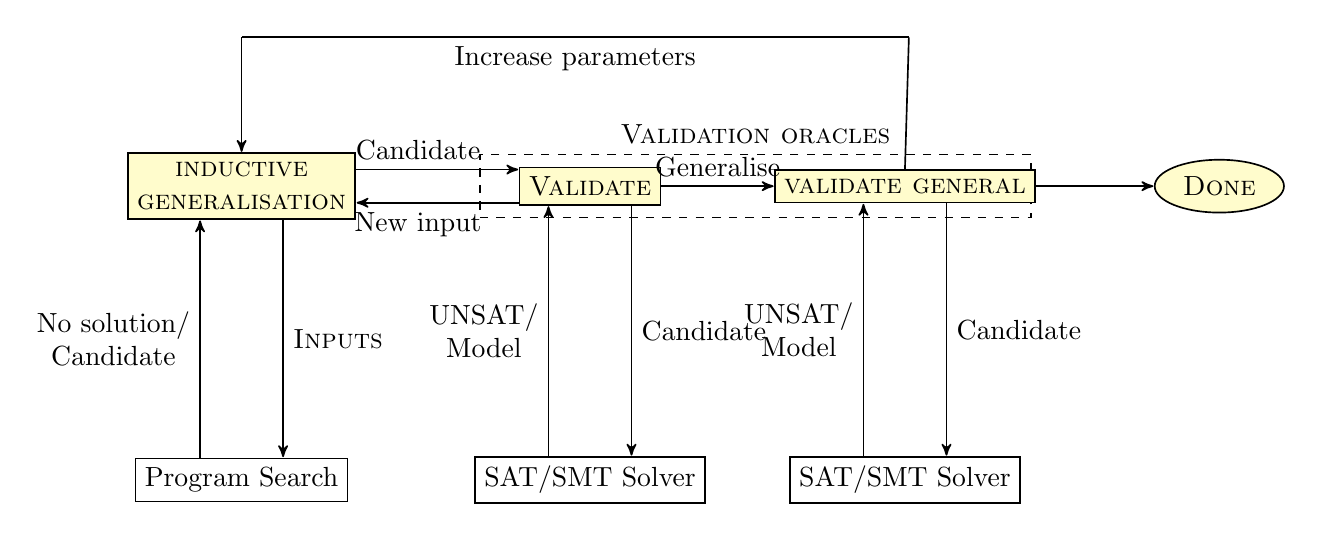
\begin{tikzpicture}[scale=0.3,->,>=stealth',shorten >=.2pt,auto, semithick, initial text=, ampersand replacement=\&,]
  \matrix[nodes={draw, fill=none, shape=rectangle, minimum height=.2cm, minimum width=.2cm, align=center
},
          row sep=1cm, column sep=1.5cm] {
   \coordinate (aux1);
   \& \coordinate (aux2);
   \& ;\\
   \node[fill=yellow!20,align=center] (synth) {{\sc inductive}\\{\sc generalisation}};
   \&
   complexnode/.pic={ 
     \node[rectangle,draw,dashed,
	minimum width=7cm,
	minimum height=.8cm,
	label={\sc Validation oracles},] (verif) {};
   \node[fill=yellow!20] (verif1) at ([xshift=-2.1cm]verif.center) {{\sc Validate}};
   \node[fill=yellow!20,align=center] (verif2) at ([xshift=1.9cm]verif.center) {{\sc validate general}};
   } 
   \& \node[ellipse, fill=yellow!20] (done) {{\sc Done}};\\
   %% \node[fill=yellow!20] (verif) {{\sc ~~~~~~Uncertainty~~~~~~}};
   %% \&
   %% \node[fill=yellow!20] (verif2) {{\sc ~~~~~~Precision~~~~~~~}};\\
   \& \\
   \& \\
   \node (gp) {Program Search};
   \&
   complexnode/.pic={ 
     \coordinate (aux);
   \node (bmc) at ([xshift=-2.1cm]aux.center) {SAT/SMT Solver};
   \node (fp)  at ([xshift=1.9cm]aux.center) {SAT/SMT Solver};
   }   
    \\
  };

   \path
    ([yshift=2em]synth.east) edge node[xshift=-0.7em] {Candidate} ([yshift=2em]verif1.west)
    ([yshift=-2em]verif1.west) edge node[xshift=-0.7em] {New input} ([yshift=-2em]synth.east)
    (verif1) edge node {Generalise} (verif2)
    ([xshift=5em]verif1.south) edge node[align=center] {Candidate} ([xshift=5em]bmc.north)
    ([xshift=5em]verif2.south) edge node[align=center] {Candidate} ([xshift=5em]fp.north)
    ([xshift=-5em]bmc.north) edge node[align=center]  {UNSAT/\\Model} ([xshift=-5em]verif1.south)
    ([xshift=-5em]fp.north) edge node[align=center]  {UNSAT/\\Model} ([xshift=-5em]verif2.south)
    (verif2) edge node {} (done)
    ([xshift=5em]synth.south) edge node[align=center] {{\sc Inputs}} ([xshift=5em]gp.north)
    ([xshift=-5em]gp.north) edge node[align=center] {No solution/\\Candidate} ([xshift=-5em]synth.south)
    (aux1) edge (synth.north);
   \path[-]
   (verif2.north) edge node[align=center] {} ([xshift=6.5cm]aux2)
   ([xshift=6.5cm]aux2) edge node[align=center] {Increase parameters} (aux1);

\end{tikzpicture}
\caption{The CEGIS loop with solution generalisation\label{fig:CEGIS-multiple-verif}}
\end{figure}

\section{Related works}

\paragraph{CEGIS}

Program synthesis is the problem of computing correct-by-design programs
from high-level specifications, and algorithms for this problem have made
substantial progress in recent years.  One such
approach~\cite{itzhaky2010simple} inductively synthesizes invariants to
generate the desired programs.

Program synthesisers are an ideal fit for synthesis of parametric
controllers since the semantics of programs capture effects such as FWL
precisely.  In~\cite{DBLP:conf/cdc/RavanbakhshS15}, the authors use CEGIS
for the synthesis of switching controllers for stabilizing continuous-time
plants with polynomial dynamics.  The work extends to its application on
affine systems, finding its major challenge in the hardness of solving
linear arithmetic with the state-of-the-art SMT solvers.  Since this
approach uses switching states instead of linear dynamics in the digital
controller, it entirely circumvents the FWL problem.  It is also not
suitable for the kind of control we seek to synthesize.  We require a
combination of a synthesis engine with a control verification tool that
addresses the challenges presented here in the form of FWL effects and
stability measures for LTI SISO controllers.  We take the former
from~\cite{DBLP:conf/lpar/DavidKL15} and the latter from~\cite{daes20161}
while enhancing the procedure by evaluating the quantization effects of the
Hardware interfaces (ADC/DAC) to obtain an accurate discrete-time FWL
representation of the continuous dynamics.

\bibliographystyle{abbrv}
\bibliography{paper}  
%\begin{thebibliography}{4}
%\end{thebibliography}


\end{document}
